\documentclass{beamer}
% Try the class options [notes], [notes=only], [trans], [handout],
% [red], [compress], [draft] and see what happens!

% \usepackage{definitions}
\usepackage[british]{babel}
\usepackage{color, soul}
\usepackage{tikz}

%% tikz tricks
% \tikzset{onslide/.code args={<#1>#2}{%
%   \only<#1>{\pgfkeysalso{#2}} 
% }}

\pdfinfo{
        /Title (cim)
        /Creator (LaTeX)
        /Producer (pdflatex)
        /Author (szerzo)
        /CreationDate (datum)
	/Subject (tema)
}


\mode<article> % only for the article version
{
  \usepackage{fullpage}
  \usepackage{hyperref}
}
\mode<presentation>
{
  \usetheme[left,width=0.65in,height=0.55in]{Kolozsvar}
  \setbeamercovered{transparent}
  \setbeamertemplate{navigation symbols}{}
  \setbeamertemplate{footline}%
     {\vspace*{-1.4em}\hspace*{0.66in}\textbf{\insertframenumber/\inserttotalframenumber}\newline\vspace*{0.4em}}
		\setbeamerfont{block title}{size=\larger} % RELSIZE -- html-sizes 
		\usefonttheme{professionalfonts}
		\setbeamercolor{math text}{fg=green!30!red!30!brown}
		\setbeamercolor{normal text in math text}{parent=math text}
}

\setbeamercovered{dynamic}

% The following info should normally be given in you main file:
\title[SonarQube Cloud]{SonarQube Cloud}
\subtitle{formerly SonarCloud}
%
\author{Hunor Ördög, Norbert-Raymond Pap, István-Lehel Balázs}
%
\institute[UBB Cluj-Napoca]{
  Department of Mathematics and Informatics\\
  Babe{\c{s}}--Bolyai University, Cluj-Napoca}
%
\date{2024 November}


\begin{document}

\frame{\maketitle}

\mode<presentation>
{
  % \begin{frame}
  %   \frametitle{Talk structure}
  % \tableofcontents
  % \end{frame} 

  % \AtBeginSection[]
  {
      \begin{frame}<beamer>{Contents}
        % \tableofcontents[currentsection,currentsubsection,hideothersubsections]
        \tableofcontents
      \end{frame}
    }
}

%%%%%%%%%%%%%%%%%%%%%%%%%%%%%%%%%%%%%%%%%%%%%%%%%%%%%%%%%%%%%%%%%%%%%%

\section[Brand changes - 28 oct 2024]{Brand changes - 28 oct 2024}

\begin{frame}{Brand changes - 28 oct 2024}
  \hspace*{2.3em}
  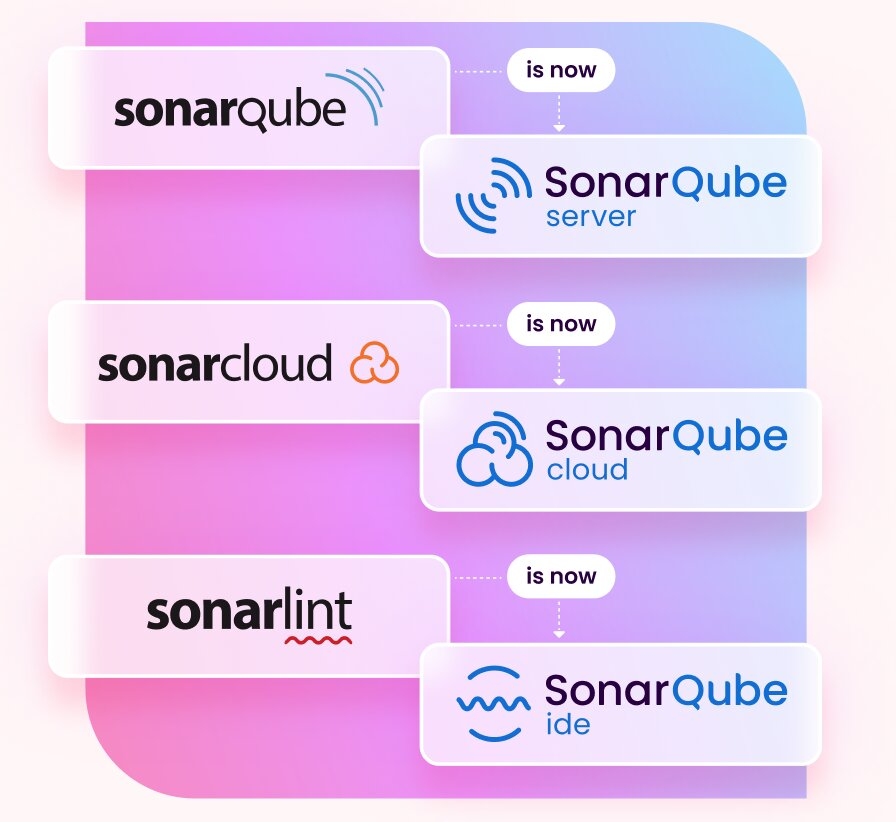
\includegraphics[scale=0.25]{fig/sonar-rebrand-1.jpg}
\end{frame}


\section[Introduction]{Introduction}

\begin{frame}{What is Sonar?}
  \begin{itemize}
    \item Tool for \textbf{code quality} and \textbf{security} throughout the development lifecycle.
    \item Catch \textbf{bugs}, \textbf{vulnerabilities}, and \textbf{design issues} 
    (Duplicated code, Large methods, Inconsistent naming).
    \item Improve \textbf{maintainability}, \textbf{readability}, and \textbf{security}.
  \end{itemize}
\end{frame}

\begin{frame}{What is Sonar?}
  \href{https://youtu.be/xeTwG9XFFTE}{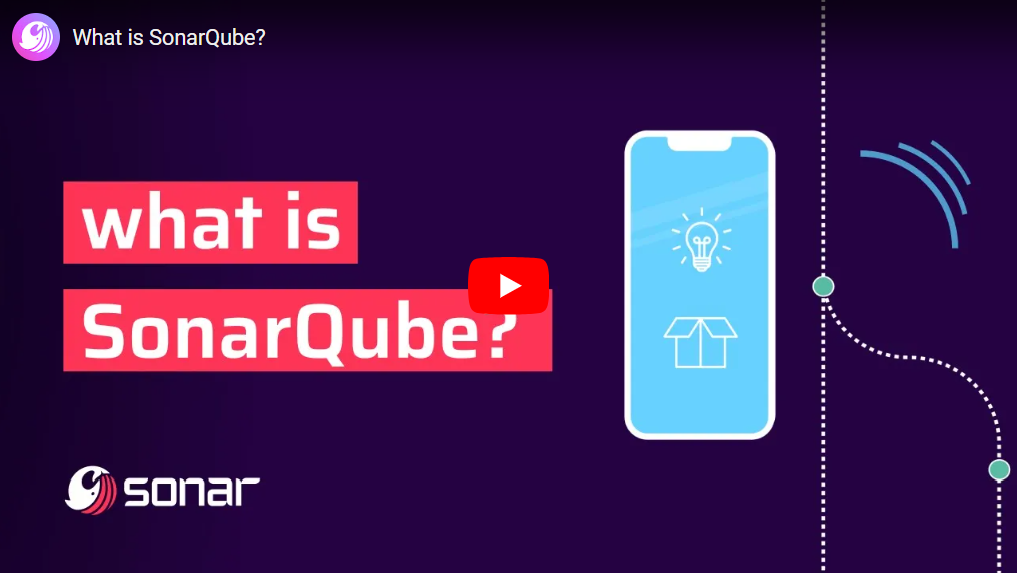
\includegraphics[scale=0.45]{fig/what_is_sonar_video.png}}
\end{frame}


\section[Why Use SonarCloud?]{Why Use SonarCloud?}

\begin{frame}{Importance of Code Quality}
  \begin{itemize}
    \item \textbf{Enhances Code Maintainability}: Ensures code is clean and structured, making future modifications easier.
    \vspace*{1em}
    \item \textbf{Prevents Technical Debt}: Identifies potential issues early to avoid accumulating maintenance burdens.
  \end{itemize}
  % \begin{tikzpicture}[remember picture, overlay]
  %   \node[left=3em] at (current page.east)
  %   {
  %     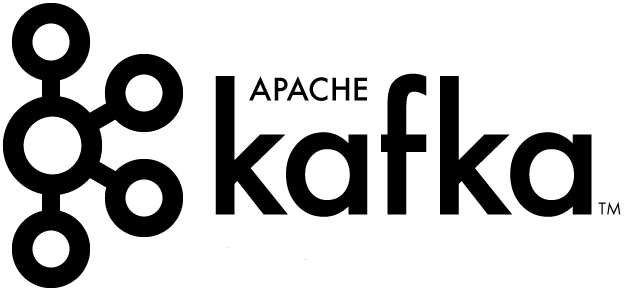
\includegraphics[width=0.35\textwidth]{fig/kafka_logo.png}
  %   };
  % \end{tikzpicture}
\end{frame}

\begin{frame}{Importance of Code Quality}
  \begin{itemize}
    \item \textbf{Reduces Defects and Bugs}: Early detection of code issues minimizes the chance of runtime errors.
    \vspace*{1em}
    \item \textbf{Improves Team Collaboration}: Sets a standard for quality, enabling consistent and effective code reviews.
  \end{itemize}
\end{frame}

\begin{frame}{Importance of Code Quality}
  \begin{itemize}
    \item \textbf{Facilitates Learning and Growth}: Promotes best practices, reinforcing sound coding principles for developers.
  \end{itemize}
\end{frame}


\begin{frame}{Security Benefits}
  \begin{itemize}
    \item \textbf{Vulnerability Detection}: Sonar identifies security vulnerabilities and potential exploits in your code, helping prevent data breaches and security incidents.
    \vspace*{1em}
    \item \textbf{OWASP Compliance}: Ensures code adheres to recognized security standards like OWASP Top 10, promoting industry-level security practices.
    % \item \textbf{Continuous Monitoring}: Provides ongoing code analysis in real-time, allowing teams to detect and fix security issues during development.
  \end{itemize}
\end{frame}

\begin{frame}{Security Benefits}
  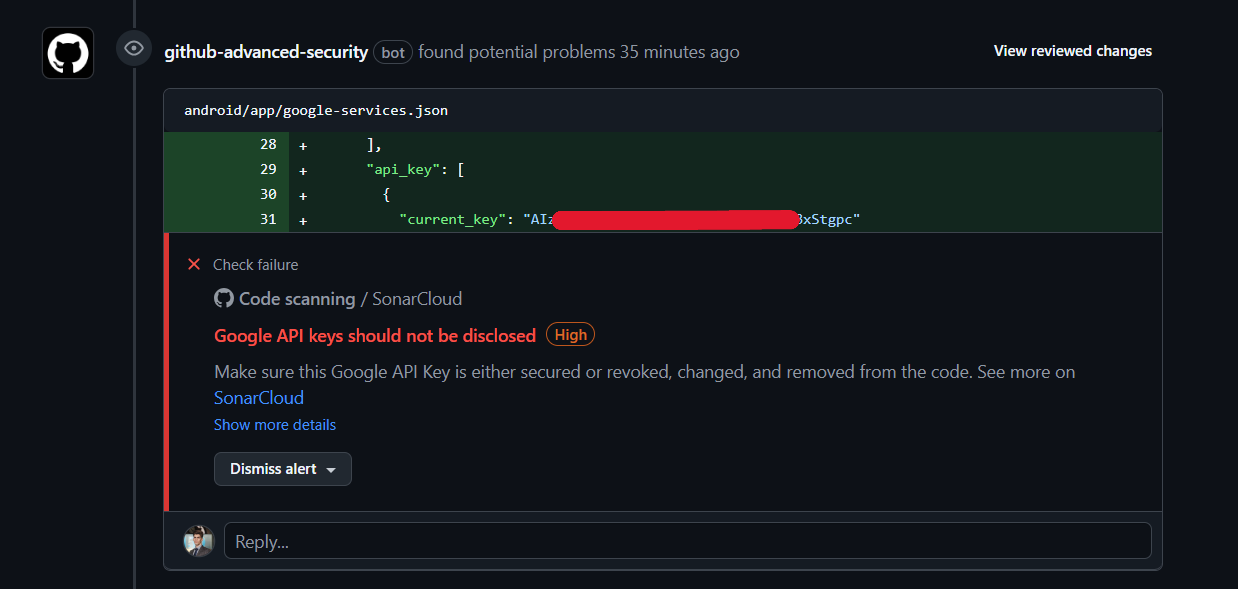
\includegraphics[width=1\textwidth]{fig/api-security-1.PNG}
\end{frame}

\begin{frame}{Security Benefits}
  \begin{itemize}
    \item Solution sugestion in SonarCloud: 
  \end{itemize}
  \vspace*{2em}
  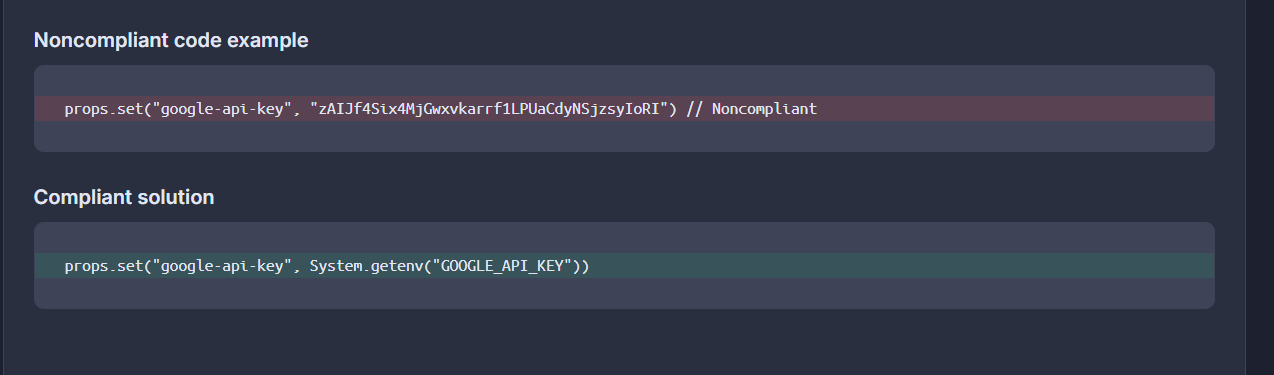
\includegraphics[width=1.04\textwidth]{fig/api-security-2.PNG}
\end{frame}

\begin{frame}{Development Best Practices}
  \begin{itemize}
    \item \textbf{Code Smell Detection}: Highlights suboptimal code structures that could lead to future maintenance problems.
    \vspace*{0.75em}
    \item \textbf{Enforces Coding Standards}: Automates the application of style and quality guidelines, ensuring consistency across the codebase.
    \vspace*{0.75em}
    \item \textbf{Automated Quality Gates}: Sets pass/fail criteria for code quality, allowing only compliant code to merge into main branches, maintaining high development standards.
  \end{itemize}
\end{frame}


\section[Key Features]{Key Features}

\begin{frame}{Code Analysis}
  % 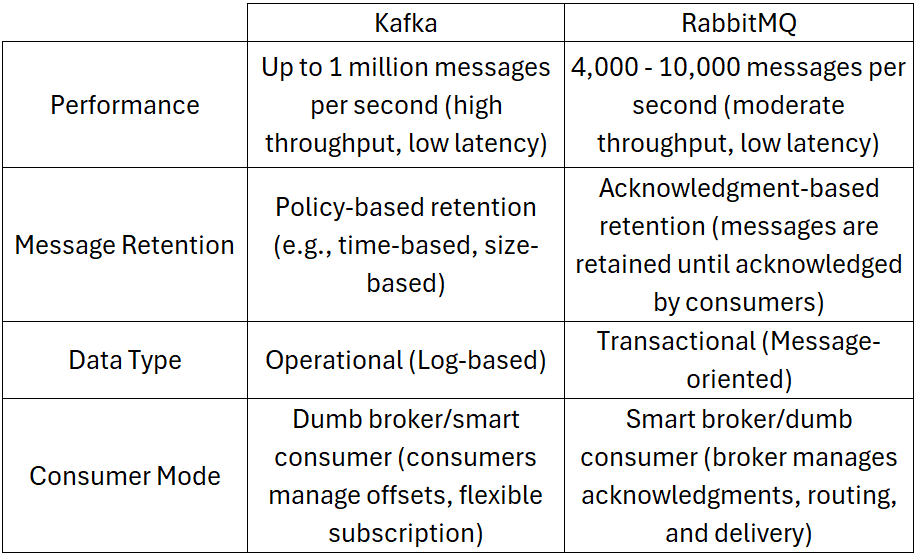
\includegraphics[width=1.02\textwidth]{fig/vs1.png}
\end{frame}

\begin{frame}{Supported Languages by SonarCloud}
  \begin{itemize}
      \item \textbf{Programming Languages:}
      \begin{itemize}
          \item ABAP, C, C++, C\#, Dart, Go, Java, JavaScript, Kotlin, PHP, Python, Ruby, Swift, TypeScript
      \end{itemize}
      \vspace*{0.5em}
        \item \textbf{Markup and Configuration:}
      \begin{itemize}
        \item CSS, SCSS, Less, style inside PHP/HTML/VueJS, HTML, XML
      \end{itemize}
      \vspace*{0.5em}
      \item \textbf{Infrastructure \& Platforms:}
      \begin{itemize}
        \item Ansible, Azure Resource Manager, CloudFormation, Docker, Kubernetes/Helm, Terraform
      \end{itemize}
      \vspace*{0.5em}
      \item \textbf{Enterprise Languages:}
      \begin{itemize}
        \item Apex, COBOL, PLI, RPG
      \end{itemize}
  \end{itemize}
\end{frame}

\begin{frame}{Integration Capabilities}
  
\end{frame}

\begin{frame}{Cloud-Based Convenience}

\end{frame}


\section[How SonarCloud Works]{How SonarCloud Works}


\begin{frame}{The Sonar Solution}
  \vspace{0.6em}
  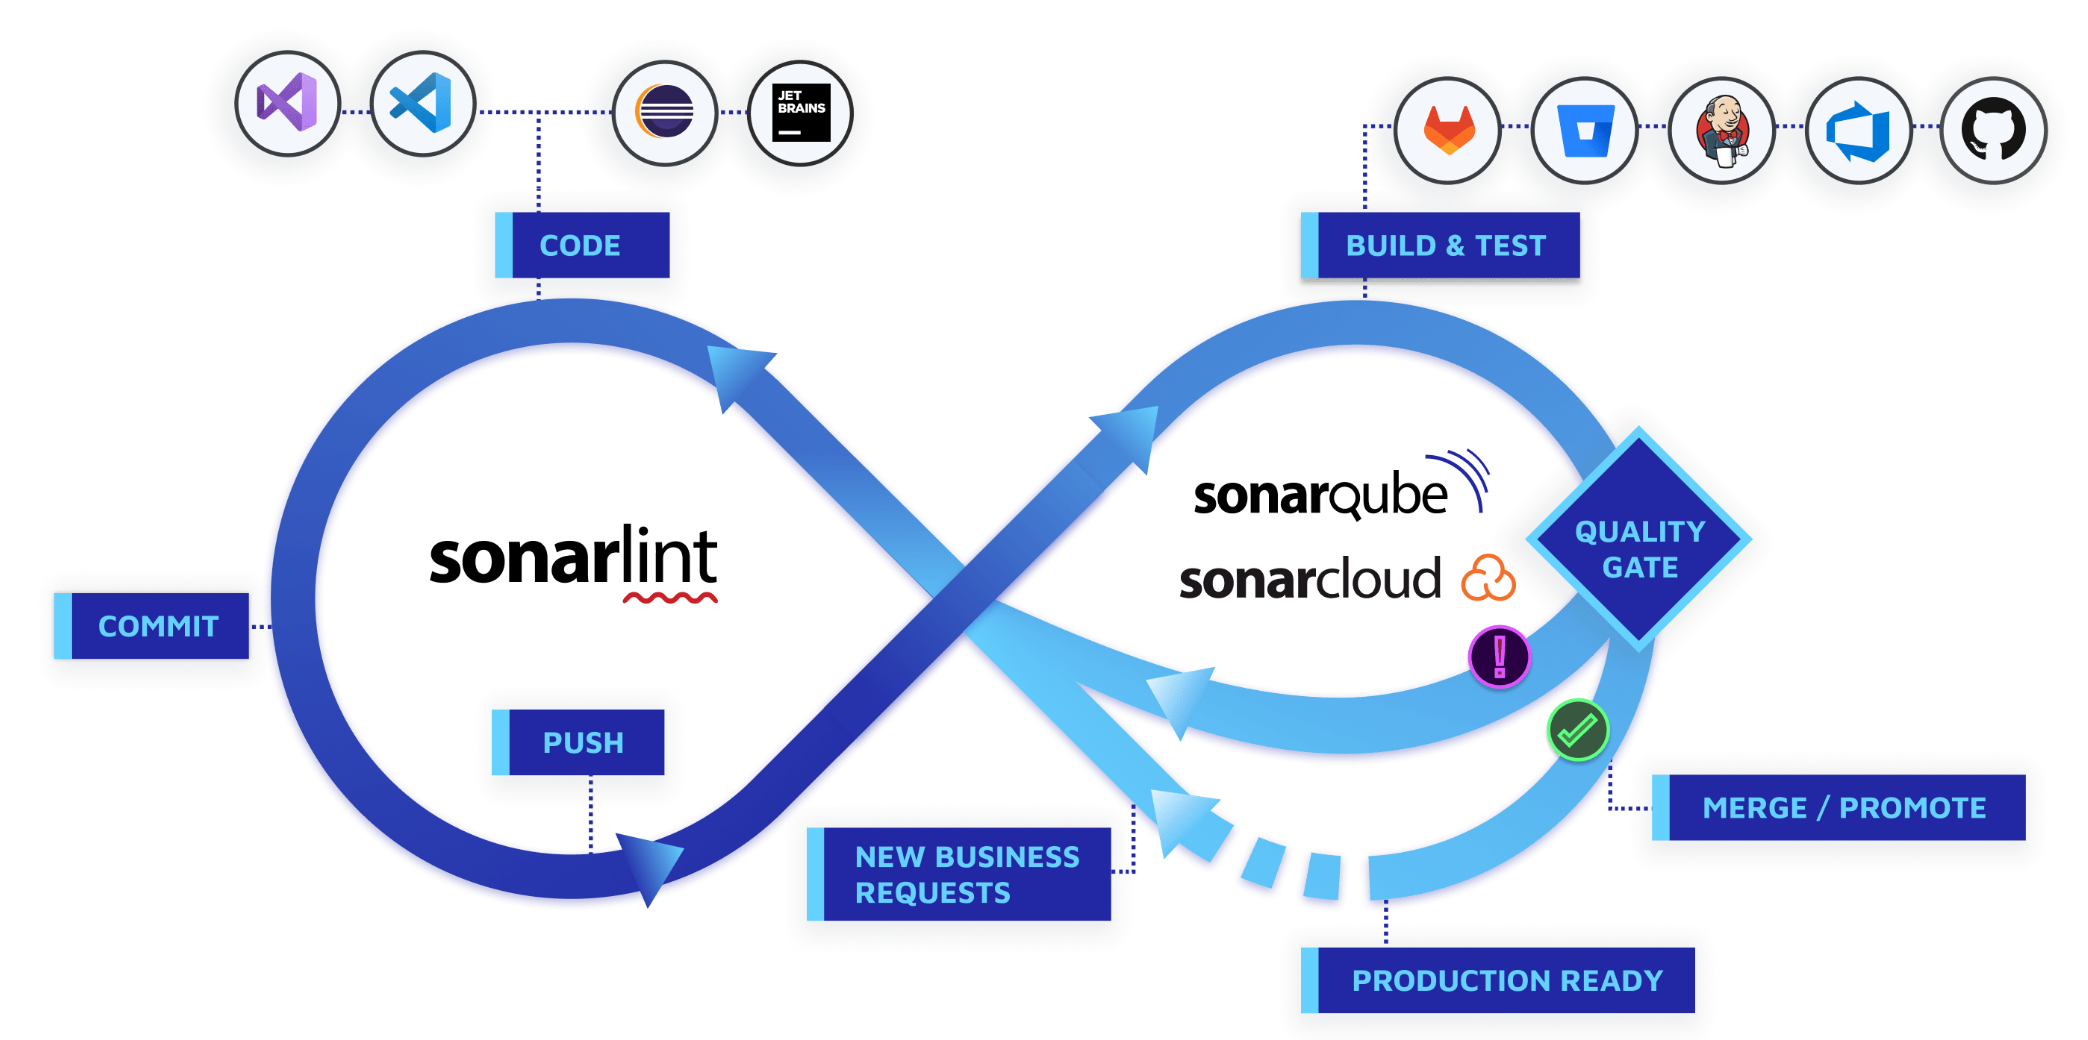
\includegraphics[scale=0.22]{fig/sonar_solution.png}
\end{frame}


\begin{frame}{Static Code Analysis}
  \begin{itemize}
    \item \textbf{Abstract Syntax Tree (AST) Parsing}: Builds a tree representation of code structure to analyze syntax and detect patterns.
    \item \textbf{Semantic Analysis}: Examines variable types, scope, and relationships between code elements to find issues like null references.
    \item \textbf{Pattern Matching with Rules}: Applies over 500 built-in rules for each language to flag common errors and risky coding patterns.
    \item \textbf{Dependency Traversal}: Analyzes code dependencies to detect unused code, duplicate functions, and inter-file issues.
\end{itemize}
\end{frame}

\begin{frame}{Quality Gates}
  \begin{itemize}
    \item \textbf{Definition:}
    \begin{itemize}
      \item Quality Gates are a set of conditions that determine whether code meets predefined quality standards.
    \end{itemize}

    \vspace*{1em}

    \item \textbf{Key Metrics:}
    \begin{itemize}
        \item \textbf{Coverage}: Enforces sufficient test coverage.
        \item \textbf{Bugs/Vulnerabilities}: Blocks critical issues.
        \item \textbf{Code Smells}: Prevents maintainability problems.
        \item \textbf{Duplications}: Limits duplicate code.
    \end{itemize}
    
    \vspace*{1em}

    \item \textbf{Outcome:}
    Pass/fail check to ensure high code standards are met.
  \end{itemize}
\end{frame}

\begin{frame}{Quality Gate - SonarCloud PR Comment}
  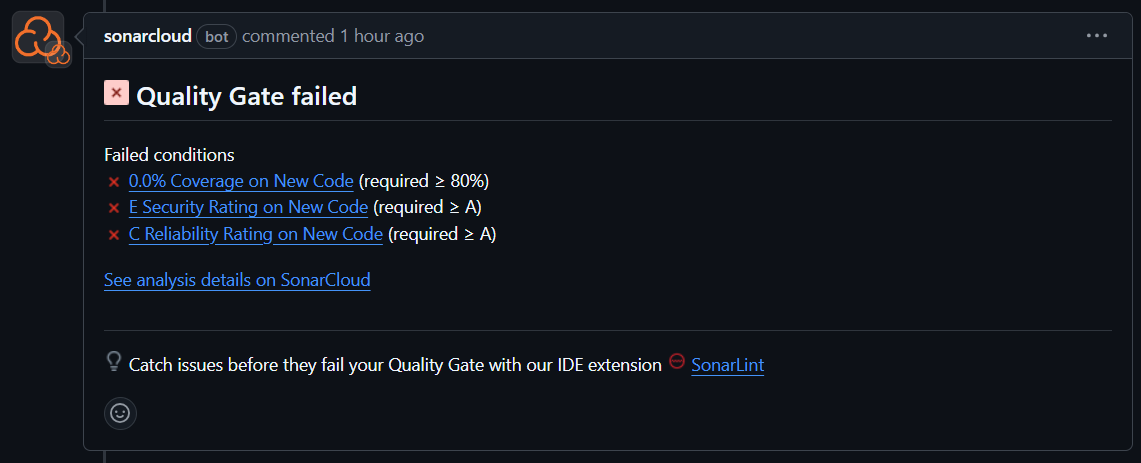
\includegraphics[width=1.0\textwidth]{fig/q-gate-1.png}
\end{frame}

\begin{frame}{Dashboard and Reports}
 
\end{frame}


\section[SonarCloud in Action]{SonarCloud in Action}

\begin{frame}{Example Workflow}
  \begin{itemize}
    \item \href{https://github.com/hunororg/ubb-flutter-pt-app/blob/main/.github/workflows/build.yml}{hunororg/ubb-flutter-pt-app/.github/workflows/build.yml}
  \end{itemize}
   
\end{frame}

\begin{frame}{Live Demo}
 
\end{frame}

\section[ Integration with GitHub and CI/CD Pipelines]{Integration with GitHub and CI/CD Pipelines}

\begin{frame}{Setting Up SonarCloud in GitHub}
 
\end{frame}

\begin{frame}{Basic Pipeline Configuration}
 
\end{frame}


\end{document}
